\section{Work Breakdown Structure}

\begin{figure}[H]
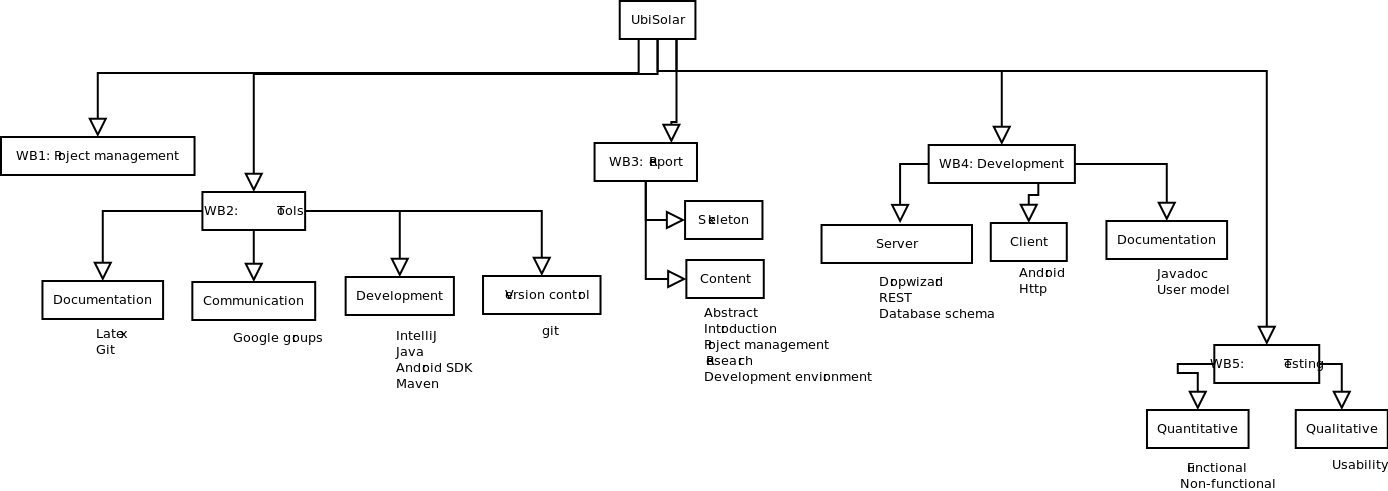
\includegraphics[width=\textwidth]{ch/planning/fig/WBS.png}
\caption{The work breakdown structure. Each WBS packet is a product of the project work.}
\label{fig:wbs}
\end{figure}

\todo[inline]{@peri: is wbs-packet correct? should it be wp (as in work package?)}

The work breakdown structure \ref{fig:wbs} is broken down into five parts. Each part is a package that represents a part of the work that needs to be done in the project.
The team decided to use WBS is so that we may analyze how much time that is actually spent on the different parts of the project, compared to how it originally was planned.
The effect of doing this is that it is easy to see whether some part of the project is forgotten or \todo[inline]{gets too much time.}

\begin{table}[H]
\centering
\rowcolors{1}{darkgray}{lightgray}
\begin{tabular}{l c r}
    \textbf{WB \#} & \textbf{Name} & \textbf{Hours} \\\hline
    1 & Project management & .5/10 = 87\\\hline
    2 & Tools 			   & 1.5/10 = 261\\\hline
    3 & Report 			   & 4/10 = 696\\\hline
    4 & Development 	   & 3/10 = 522\\\hline
    5 & Testing  		   & 1/10 = 174\\\hline
\end{tabular}
\end{table}

From the total amount of hours for project, the team has divided each WBS packet into a smaller part, based on how much time the team should use one the given part.

For each sprint the team can see how much time that has been spent on each packet, \todo{and if time is beeing distributed according to the planned amount of time on each packet.}